%%%%%%%%%%%%%%%%%%%%%%%%%%%%%%%%%%%%%%%%%%%%%%%%%%%%%%%%%%%%%%%%%%%%%%%%%%%%%%%%%%
% NAME:		swift_scijust_template.tex
% LANGUAGE:	LaTeX
% AUTHOR:	Eleonora Troja, eleonora.troja@nasa.gov
% CREATED:	2014-08-01
% MODIFIED:	2015-08-01
%%%%%%%%%%%%%%%%%%%%%%%%%%%%%%%%%%%%%%%%%%%%%%%%%%%%%%%%%%%%%%%%%%%%%%%%%%%%%%%%%%
%% LaTeX template for the science justification & technical feasibility
%% to be submitted as part of a Swift Guest Investigator proposal.
%%
%% Swift Cycle 12
%% Deadline: 25 September 2015, 4.30pm EDT
%%
%%%%%%%%%%%%%%%%%%%%%%%%%%%%%%%%%%%%%%%%%%%%%%
%%%%% Default format: 11pt single column %%%%%
%%%%%%%%%%%%%%%%%%%%%%%%%%%%%%%%%%%%%%%%%%%%%%

\documentclass[letterpaper,11pt]{article}

%%%%%%%%%%%%%%%%%%%%%%%%%%%%%%%%%%%%
%%%%% Default font, two-column %%%%%
%%%%%%%%%%%%%%%%%%%%%%%%%%%%%%%%%%%%

%\documentclass[letterpaper,11pt,twocolumn]{article

%%%%%%%%%%%%%%%%%%%%%%%%%%%%%
%%%%% Included packages %%%%%
%%%%%%%%%%%%%%%%%%%%%%%%%%%%%

\usepackage{graphics,graphicx}
\usepackage{psfig}
\usepackage{times}
\usepackage{natbib}
\usepackage{multicol}

%%%%%%%%%%%%%%%%%%%%%%%%%%%%%%%%%%%%%%%%%%%%%%%%%
%%%%% Page dimensions                       %%%%%
%%%%% DO NOT CHANGE THE FOLLOWING 9 LINES!  %%%%%
%%%%%%%%%%%%%%%%%%%%%%%%%%%%%%%%%%%%%%%%%%%%%%%%%

\setlength{\textwidth}{7in} 
\setlength{\textheight}{9.5in}
\setlength{\topmargin}{-0.2in} 
\setlength{\oddsidemargin}{-0.2in}
\setlength{\evensidemargin}{-0.2in} 
\setlength{\headheight}{0in}
\setlength{\headsep}{0in} 
\setlength{\hoffset}{0in}
\setlength{\voffset}{0in}


%%%%%%%%%%%%%%%%%%%%%%%%%%%%%%%%%%
%%%%% Section heading format %%%%%
%%%%%%%%%%%%%%%%%%%%%%%%%%%%%%%%%%

\makeatletter
\renewcommand{\section}{\@startsection%
{section}{1}{0mm}{-\baselineskip}%
{0.5\baselineskip}{\normalfont\Large\bfseries}}%
\makeatother

\newcommand{\swift}{\textit{Swift}}
\newcommand{\fermi}{\textit{Fermi}}
\newcommand{\pasp}{\textit{PASP}}
\newcommand{\apj}{\textit{ApJ}}
\newcommand{\nat}{\textit{Nature}}
\newcommand{\apjl}{\textit{ApJ}}
\newcommand{\mnras}{\textit{MNRAS}}
\newcommand{\aj}{\textit{AJ}}
\newcommand{\aap}{\textit{A\&A}}
\newcommand{\actaa}{\textit{ATCAA}}

%%%%%%%%%%%%%%%%%%%%%%%%%%%%%%%%%%%%%%%%%%%%%%%%%%%%%%%%%%%%%%%%%%%%%%%%%%%%%%%%%%
%  NOTES:
% 
%  - THE SCIENTIFIC JUSTIFICATION MUST NOT EXCEED 4 PAGES!
%     (The only exception are “Key Projects” and proposals in the "high redshift GRB" category which can have up to 6 pages)
%
%  - THE "BUDGET NARRATIVE" MUST BE LESS THAN 1 PAGE AND DOES  NOT  COUNT TOWARD THE ABOVE PAGE LIMIT
%
%  - IT IS STRONGLY RECOMMENDED TO USE A FONT SIZE OF 11pt OR LARGER.
%
%  - Do NOT include a CV, current and pending support, or any other supporting information 
%
%  - THE PROPOSAL MUST BE SUBMITTED AS A PDF  FILE:
%
%  latex swift_scijust_template.tex
%  dvips swift_scijust_template -o swift_scijust_template.ps
%  ps2pdf swift_scijust_template.ps swift_scijust_template.pdf
%
%%%%%%%%%%%%%%%%%%%%%%%%%%%%%%%%%%%%%%%%%%%%%%%%%%%%%%%%%%%%%%%%%%%%%%%%%%%%%%%%%%

\begin{document}
\pagestyle{plain}
\pagenumbering{arabic}

\begin{center} 
\bfseries\uppercase{Early and Deep Follow-up of Swift GRBs with P60
and the SED Machine}
\end{center}
\vspace{-0.3cm}
\centerline{\bf PI: {N. Konidaris}}
 
\noindent {\bf 1. Abstract}
\smallskip\\
We propose to continue our successful program of rapid, deep, multi-filter
follow-up of \textit{Swift} gamma-ray bursts (GRBs) with the Palomar 
60-inch telescope (P60).  Our science goals are to: (A) Rapidly identify 
high-redshift and highly dust-obscured GRBs; (B) conduct multi-wavelength
observations to identify reverse shocks and constrain the total energetics
of GRBs; (C) build up large, high-quality, \textit{unbiased} samples of
optical light curves and host galaxies to enable demographic studies;
(D) provide an automated, early-time spectroscopic capability to enable
immediate redshift measurement and sensitive constraints on the color 
evolution of GRBs with the SED Machine. \\


\noindent {\bf 2. Description of the Proposed Program}
\smallskip\\
The P60 telescope is one of only a handful of 2-m class facilities worldwide
equipped to robotically respond to GRBs.  The additional depth provided 
relative to smaller facilities has emerged as a critical capability in an 
era where the typical \textit{Swift} optical afterglow is only $R$$\sim$19 mag at 
$\sim$5--10 minutes after the GRB \citep{ckh+09,as+07}, often precluding 
detection with smaller telescopes.  This combination of rapid-response 
capability and depth not only enables more afterglow detections (we 
detect $\sim$80\% of GRBs which P60 is able to observe within 20 minutes) 
but also provides an immediate handle on the afterglow properties: events 
not detected by P60 have been shown almost invariably to be either heavily 
dust-extinguished or, most excitingly, at $z>5-6$ \citep{ckh+09,pcb+09}.

The promptly available and rapidly disseminated (see below) results
from P60 GRB observations enable a wide array of scientific investigations;
we describe the primary science objectives of our team below.  However, we
wish to emphasize that by publicly (e.g., via GCN Circulars) reporting our
results in a timely manner, we also enable the broader GRB
community to more intelligently plan and execute their science programs
at other (often larger-aperture) facilities. 

\noindent {\it A) Heavily extinguished and high-$z$ GRBs}:
\smallskip\\
It has long been recognized that GRBs may serve as unique probes of
the high-redshift universe, extending even into the epoch
of reionization (e.g., \citealt{lr00}).  However, much of the 
difficultly in discovering high-redshift ($z > 6$) GRBs  
has come from the large number of false positives, especially from 
dust-extinguished events.  The large aperture and red coverage 
of P60 are of considerable help in recognizing genuine high-$z$ bursts:  
the 80\% detection efficiency from prompt P60 observations 
greatly reduces a significant contaminant to high-$z$ GRB searches 
(compared to, for example, the 50\% detection rate from UVOT), enabling 
more efficient utilization of limited resources (NIR imaging and spectroscopy).  
P60 nondetections have played a central role in motivating NIR follow-up that 
directly led to the redshift measurements of two of three spectroscopically 
confirmed $z>6$ events to date, (GRB\,050904: \citealt{hnr+06}; GRB\,090423: 
\citealt{trl+09}).  Our group will continue to pursue access to NIR capabilities
on large-aperture facilities in an attempt to utilize high-redshift
events as probes of the epoch of reionization (e.g., Keck, Gemini); however, 
P60 non-detections will continue to be prime high-$z$ candidates for 
follow-up by the entire GRB community.

\noindent {\it B) Multiwavelength Modeling and Energetic GRBs}:
\smallskip\\
One of the remaining unresolved puzzles of the \swift\ era is the lack
of achromatic jet breaks indicating collimation of the relativistic outflow
\citep{kb08,rlb+09,p07}.  The resulting highly isotropic explosions have
proven to be significantly more energetic than pre-\swift\ events, with
several events exceeding a collimation-corrected energy release of
$10^{52}$\,erg (so-called ``hyper-energetic'' GRBs: \citealt{ccf+08,ckh+06};
Fig.~\ref{fig1}b).  Such a result is difficult to reconcile with the
standard ``collapsar'' model for GRBs \citep{woo93}.  
P60  will continue to provide 
detailed, multi-color light curves for \swift\ afterglows, in some cases extending 
out to weeks after the burst (Figure 1), to search for jet breaks and constrain event energetics.  
We also have a program at the VLA, enabling these events to be followed
across the electromagnetic spectrum to better constrain the properties of mildly 
relativistic ejecta that are lacking from studies based only in the X-ray and 
optical bandpasses.  Our approach has most recently been demonstrated in our
observations and modeling of the bright \swift/{\emph Fermi} GRB\,130427A \citep{pcc+2013}.

\noindent {\it C) Population Statistics for \swift\ GRBs}:
\smallskip\\
As \swift\ matures as a facility, attention has gradually shifted away from in-depth 
studies of individual events towards integrative studies of large populations of 
\swift\ bursts.  However, the heterogeneous optical follow-up of GRBs presents a challenge: 
almost half of all \swift\ GRBs do not have reported optical afterglows, and those which do 
may be biased by selective observing or reporting and complicated by the different characteristics of different telescopes.  
P60 has been accumulating a sample of sensitive, multi-color, early-to-late time 
photometry of \swift\ bursts almost from the satellite launch through the present time.
Since it is a robotic telescope, its automatically triggered events are fully unbiased by
any human decision-making.  We will continue our campaign to bolster this sample
(currently standing at 62 events, 80\% of which have detected afterglows, 65\% with
spectroscopic redshifts, and 100\% with redshift upper limits) as well as to publish an 
updated catalog to the community within the next Cycle, building upon our previous 
release \citep{ckh+09,pcb+09}.

\noindent {\it D) Rapid-Response Time-Resolved Spectroscopy}:
\smallskip\\
The SED Machine is a new P60 instrument with unique capabilities.  
While retaining the multi-color photometric follow-up capabilities of 
the previous P60 imaging camera (via its four-filter Rainbow Camera), the 
SED Machine also provides a completely new capability in the form of its 
26$\times$26'' low-resolution IFU (Figure 2).  The SED Machine can respond 
immediately to new GRBs to provide early photometric coverage and, once an X-ray 
position is acquired, the afterglow will be positioned onto the IFU for 
immediate spectroscopy.  While the resolution $R$$\sim$100 is too low to 
provide traditional spectroscopic redshifts from metal lines, the SED Machine 
will be able to instantly recognize Lyman breaks (and DLAs) for GRBs at $2 < z < 6$, 
providing firm, precise redshift measurements without having to resort to 
observationally-intensive triggers on larger telescopes.  In addition, by taking 
multiple exposures on the same source, the SED machine will provide a time-resolved 
window on optical color changes starting at very early times, providing 
simultaneous color measurements from $\lambda=370-920$\,nm enabling the most 
detailed look yet at early-time color changes from both intrinsic GRB processes 
(evolution of the afterglow) and extrinsic ones (dust photodestruction). \\

\noindent {\bf 3. Justification of Requested Observing Time, Feasibility, and Visibility}
\smallskip\\
We expect to be able to respond to $\sim 6$ afterglows within an hour of the burst
trigger with P60 over the course of Cycle 12 (based on numbers observed during 
previous cycles).  Given P60 sensitivity limits ($R < 20.5$\, mag in 60\,s; 
$R < 23$\,mag in 1\,hr), all P60 identified afterglows will be suitable for 
follow-up optical spectroscopy on large facilities (e.g., Keck, Gemini) and, in 
many cases, late-time follow-up with P60 and with larger telescopes to monitor 
the light curve and build multi-wavelength SEDs.  

Of the 6 GRBs with prompt P60 response, we expect $\sim 1-2$ will have
no P60 detection and therefore be considered robust high-z or dark 
burst candidates.  These events will be targeted for detailed studies
in the NIR of the afterglow and/or host galaxy.  At the other extreme, 1--2 
afterglows per year will be sufficiently optically bright for long-term 
follow-up and energetics studies.

The SED Machine was commissioned in summer 2013 and is now available; 
during Cycle 12 it will alternate time on the telescope with the existing 
imaging camera.  The SED Machine IFU
reaches S/N$>$6 per resolution element down to $V \sim 20.5$ mag in 20 minutes,
which should be sufficient to provide redshifts (or redshift upper limits) 
for at least $\sim$50\% of GRBs given the brightness distribution 
(2--4 events in Cycle 12 after installation).  Any GRBs not detected at any 
wavelength on the IFU after 20 minutes (1--3 events) will be sent back to 
imaging with the Rainbow Camera and (if still undetected) pursued vigorously 
with other facilities as candidate dark bursts following the strategy outlined 
previously.

While the SED Machine instrument is meeting its performance goals, funding 
provided by this proposal will allow us to develop a \textit{real-time,
fully automated data reduction pipeline} for the IFU.  With this in place,
we can promptly notify the entire GRB community of the results from the
SED machine so that they can schedule follow-up observations (e.g.,
NIR imaging/spectroscopy for high-$z$ candidates) appropriately.

We do not request any additional \swift\ observations for our program. \\

\noindent {\bf 4. Justification of Duplication} %Only for observing proposals
\smallskip\\
We are proposing for funding to support ground-based observations of new GRBs, so 
there are no duplications.\\

\noindent {\bf 5. Report on Previous Swift and Related Programs}
\smallskip\\
We have previously been awarded funding from \swift\ for rapid optical
follow-up with P60 in Cycles 1, 2, 4, and 5.  The results of this work are best
examined through the relevant publications (section 6) and GCN circulars.  
While P60 GRB operations have not been funded since 2009, we have made a 
concerted effort to continue our operations and rapidly announce results
to the community: we have published 22 GCN circulars from P60 during the last 
12 months; 
major recent results include a detailed study of the bright 
\swift\ GRB\ 130427A, which rapidly triggered and was extensively observed by 
P60  \citep{pcc+2013} as well as follow-up of the afterglow
and supernovae associated with nearby GRBs 130702A \citep{sck+13,tcs+15} and 
140606B \citep{skc+15,cdp+15}.  
With the coming switch from the current camera to routine observations with 
the SED machine further support is critical for this effort to continue.
\\


\noindent {\bf 6. References}
\smallskip\\
\begin{multicols}{2}
{\footnotesize
\bibliographystyle{apjprop}
\bibliography{journals_apj,mastergrb,gcn}
}
\end{multicols}

\noindent {\bf 7. Budget Narrative} % Only for funding proposal
\smallskip\\
The current arrangement with Caltech Optical Observatories requires that
users of P60 support operations through the science programs
utilizing the telescope. We therefore request partial support for
our expected fraction of P60 usage ($10\%$, \$20K) and an additional \$10K 
for postdoc or student support to implement an updated triggering and rapid-reduction
pipeline for SED machine follow-up of GRBs.
This support ensures
that P60 will be able to place {\em Swift} GRB followup as its
highest scientific priority and to ensure a seamless transition in ToO operations
between the current camera and the SED Machine.

Additionally, we request partial summer salary for co-I Harrison (\$2K) and
co-I Kulkarni (\$2K), travel support for PI Perley and co-I Cenko
(\$3K), and associated research costs (\$3K) including publication of an
updated P60 afterglow catalog.  These numbers are inclusive of overhead. 

%-----------------------------Figure Start------------------------------
\begin{figure}[htp!]
\begin{center}
\hbox{
 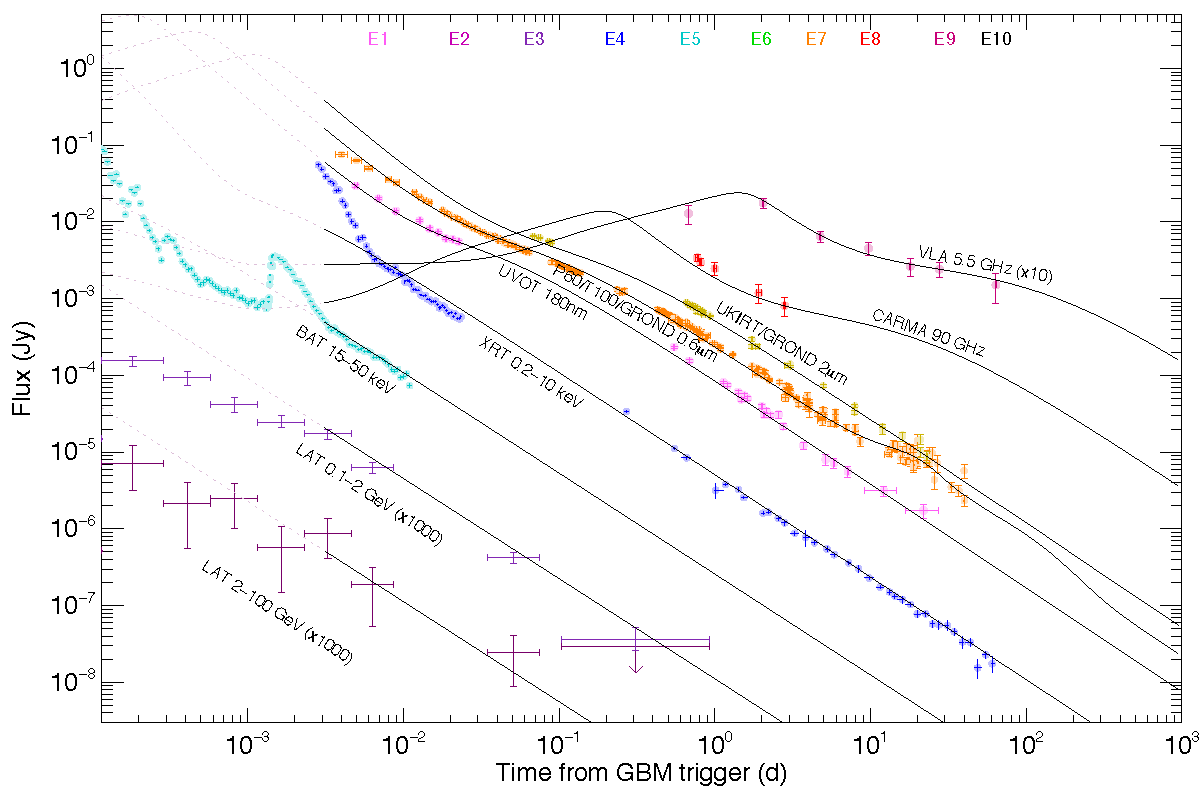
\includegraphics[width=0.5\textwidth]{130427a.pdf}
 \hspace{0.5cm}
 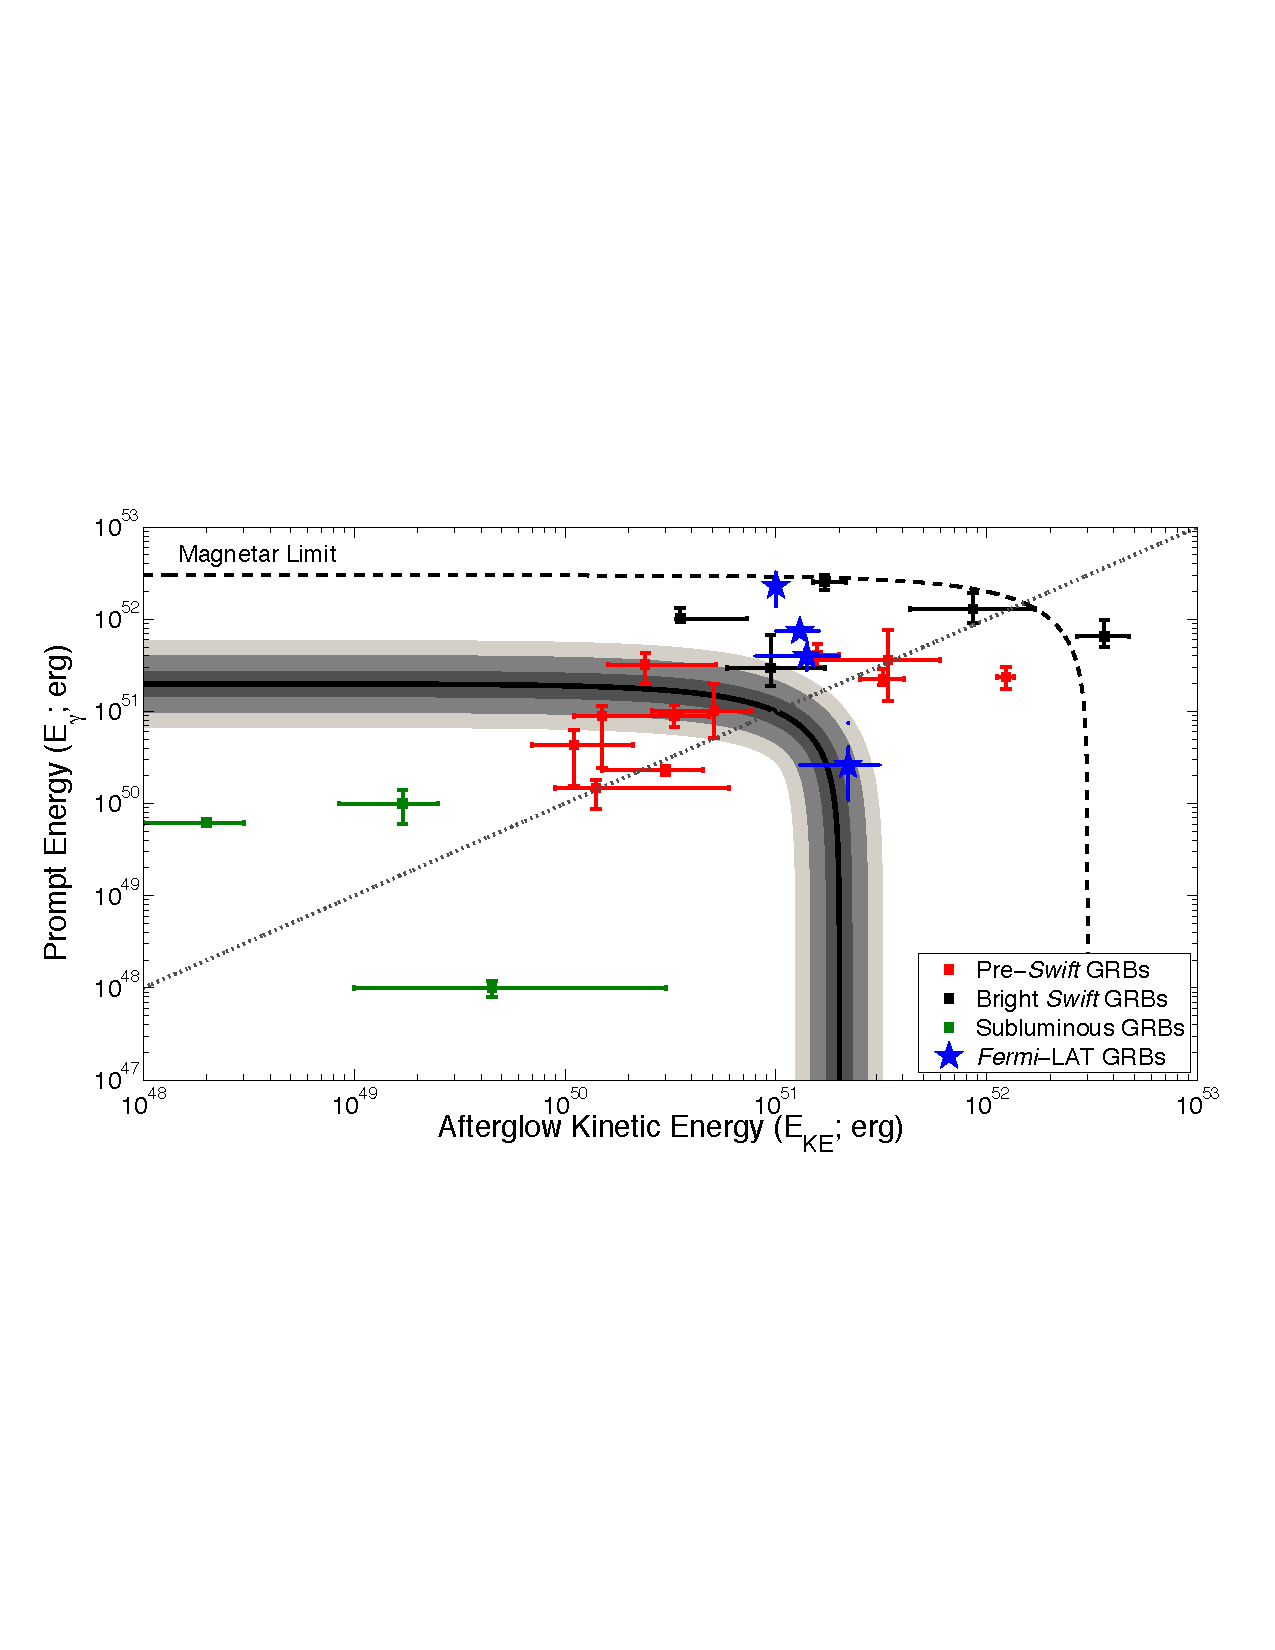
\includegraphics[width=0.5\textwidth]{waterfall_lat.pdf}
 }
\end{center}
\caption{\footnotesize
{{\it (a) Left panel}:  Multiwavelength observations and modeling of GRB 130427A (from Perley et al.\ 2013).  
Most of the $r$-band observations (as well as $g$,$r$, and $z$; not shown) were provided by P60.  Radio observations were provided (in part) by our programs at VLA and CARMA.  With this combined data set we were able to constrain the GRB properties (e.g., shockwave energy, microphysics) and environment (density structure) in detail and demonstrate the presence of a bright multiwavelength reverse shock.
{\it (b) Right panel}: Two-dimensional relativistic energy release ($E_{\mathrm{rel}} \approx
E_{\gamma} + E_{\mathrm{KE}}$) from GRBs.  Cosmologically distant ($z > 0.5$)
events from the pre-\swift\ era are shown in red.  The logarithmic mean
for these events, $\langle E_{\mathrm{rel}} \rangle = 2 \times 10^{51}$\,erg, is 
indicated by the solid black line.  Shaded regions correspond to 1$\sigma$, 2$\sigma$,
and 3$\sigma$ errors on this mean value.  Nearby underluminous events (GRBs\,980425, 031203,
and 060218) are plotted in green.  We have further identified a class of bright \swift\ and \fermi\
events that are over-luminous, with total energy release in excess of $10^{52}$\,erg.  Such
hyper-energetic events pose a severe challenge to magnetar models.}}
\label{fig1}
\end{figure}


\begin{figure}[ht!]
\begin{center}
\hbox{
 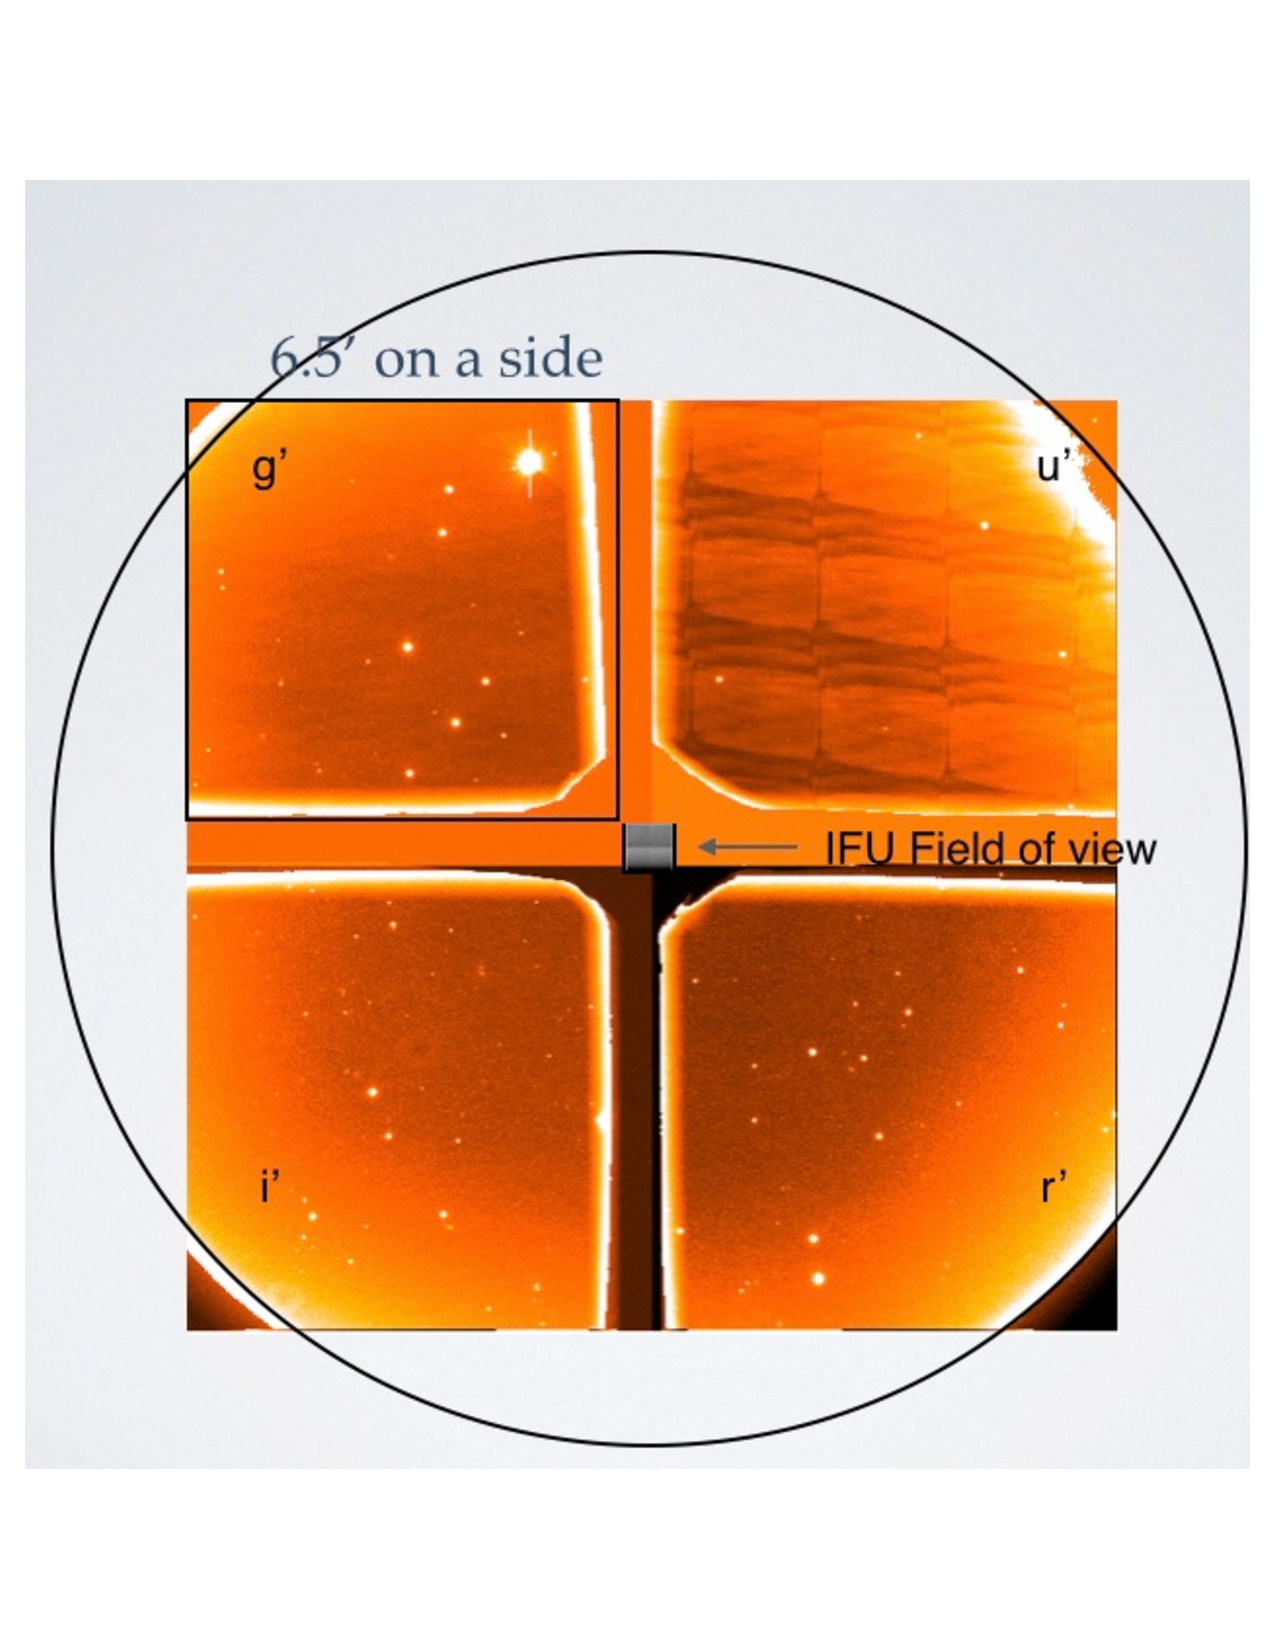
\includegraphics[width=0.4\textwidth]{SEDM.pdf}
 \hspace{0.5cm}
 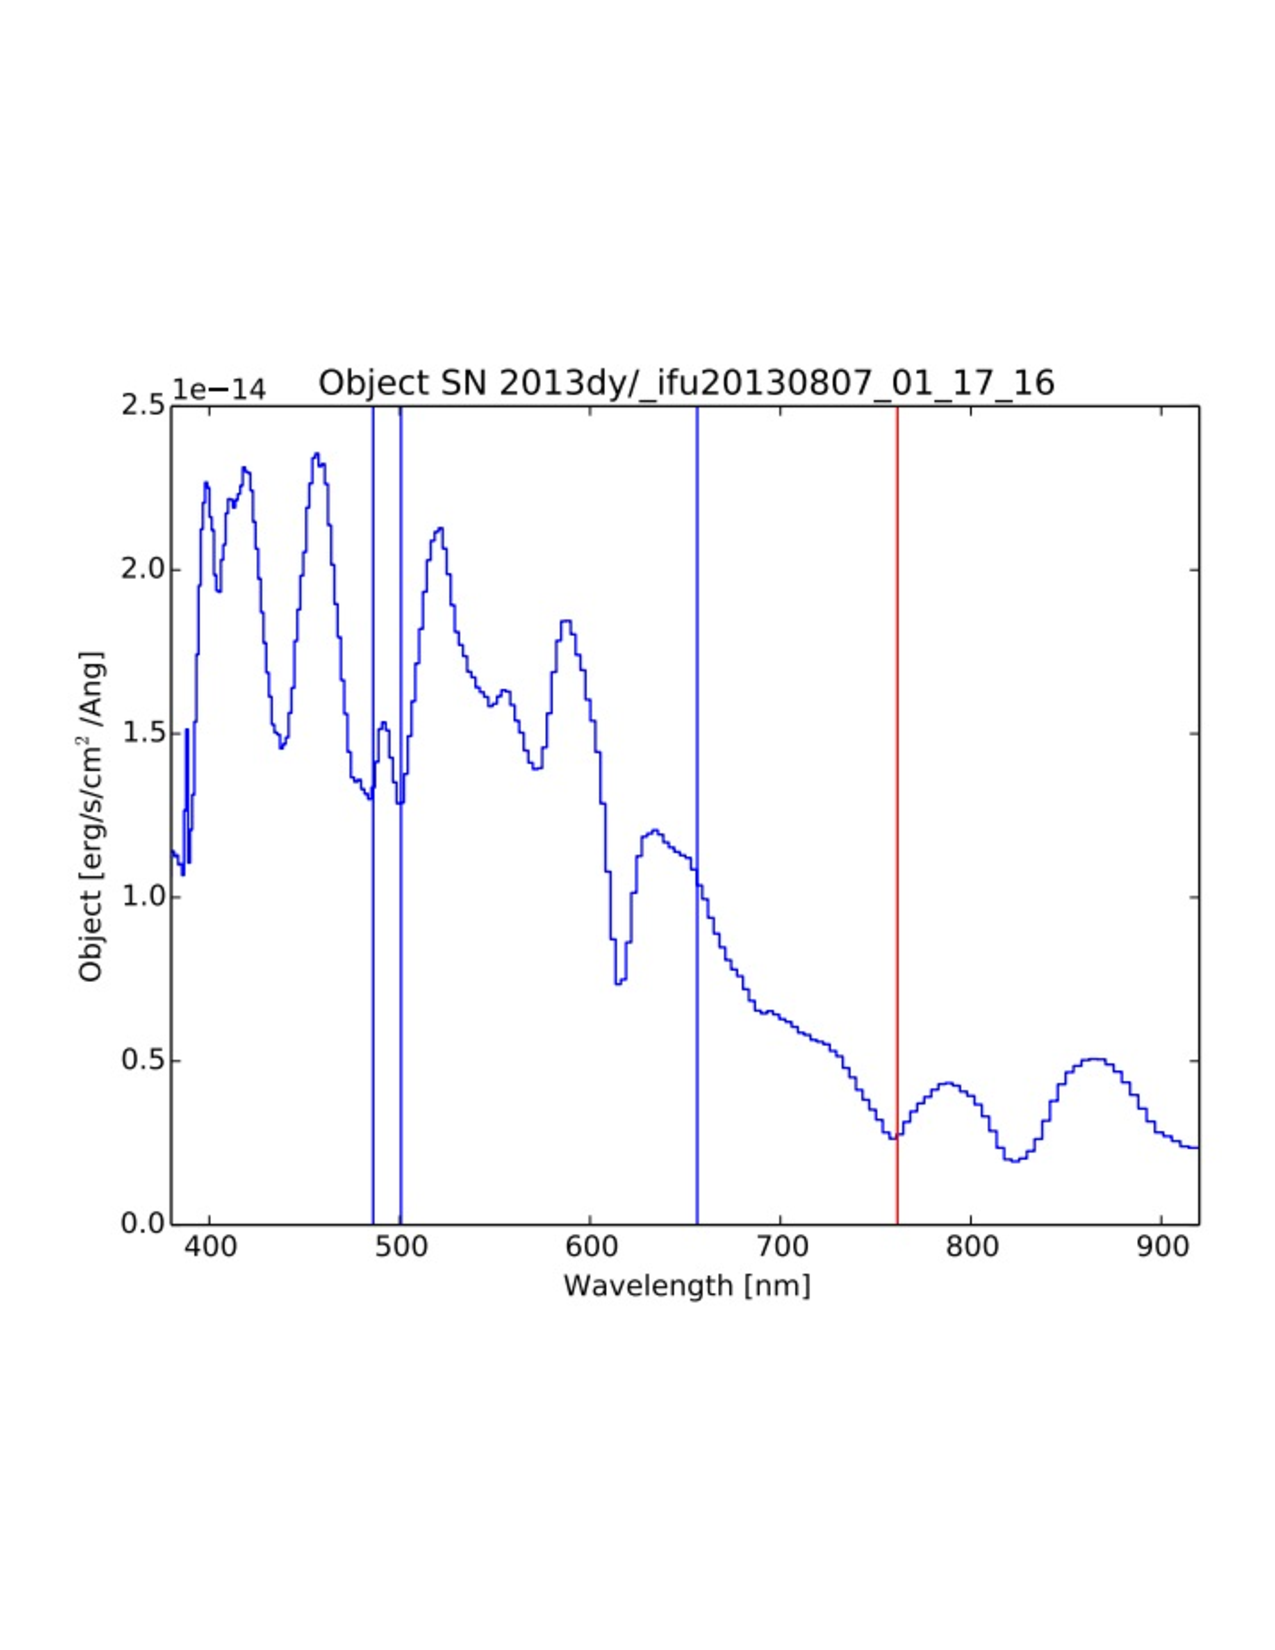
\includegraphics[width=0.5\textwidth]{SN2013dy.pdf}
 }
\end{center}
\caption{\footnotesize
{{\it (a) Left panel}: Focal plane layout of the SED machine, a combined imager 
(the four-filter Rainbow Camera) and IFU low-resolution spectrograph.  BAT positions 
will be first be sent to the $r$-band quadrant of the Rainbow Camera for early 
light curve information, then (when the XRT position is distributed) the afterglow 
will be sent to the IFU to provide an immediate spectroscopic redshift as well as 
time-resolved $R\sim100$ spectroscopy to constrain the afterglow's early color 
evolution. {\it (b) Right panel}: SED Machine spectrum of the type Ia supernova
SN2013dy, obtained during commissioning in August 2013. The SED Machine IFU
reaches S/N$>$6 per resolution element down to $V \sim 20.5$ mag in 20 minutes,
which should be sufficient to provide redshifts (or redshift upper limits) for
the majority of \textit{Swift} GRBs.}}
\label{fig2}
\end{figure}



\end{document}
